\documentclass[10pt,aspectratio=169]{beamer}
\usepackage[utf8]{vietnam}
\usepackage{fil}

\title{Mô phỏng thuật toán Reinforcement Learning cho Serverless}
\subtitle{Future Internet Laboratory}
\author{Nguyễn Phạm Trung Hiếu}

\begin{document}

\maketitle

\begingroup
    \begin{frame}{Nội dung chính}{}
        \tableofcontents
    \end{frame}
\endgroup

\section{Kịch bản mô phỏng}

\begin{frame}{Điều kiện thay đổi trạng thái}{\secname}
\begin{itemize}
\setlength\itemsep{8pt}
\item Giới hạn sự thay đổi state chỉ giữa hai state liền kề, state chỉ thay đổi một mức mỗi lần.
\item Biểu diễn ma trận đơn vị $ M_u $ theo cách hiểu khác (nói thêm ở vấn đề gặp phải):
\begin{itemize}
\setlength\itemsep{4pt}
\item[-] -1: state nguồn, tương ứng với state bị thay đổi
\item[-] 1 : state đích, tương ứng với state thay đổi tới
\item[-] 0 : state không bị thay đổi
\end{itemize}
\item[] $ \longrightarrow $ Hai giá trị -1 và 1 luôn liền kề nhau (nếu có thay đổi ở hai vị trí state thì -1 và 1 sẽ được xếp theo từng cặp).
\end{itemize}
\end{frame}

\begin{frame}{Điều kiện thay đổi trạng thái}{\secname}
\begin{center}
\textbf{\small Trường hợp thoả mãn}\\
\vspace{4pt}
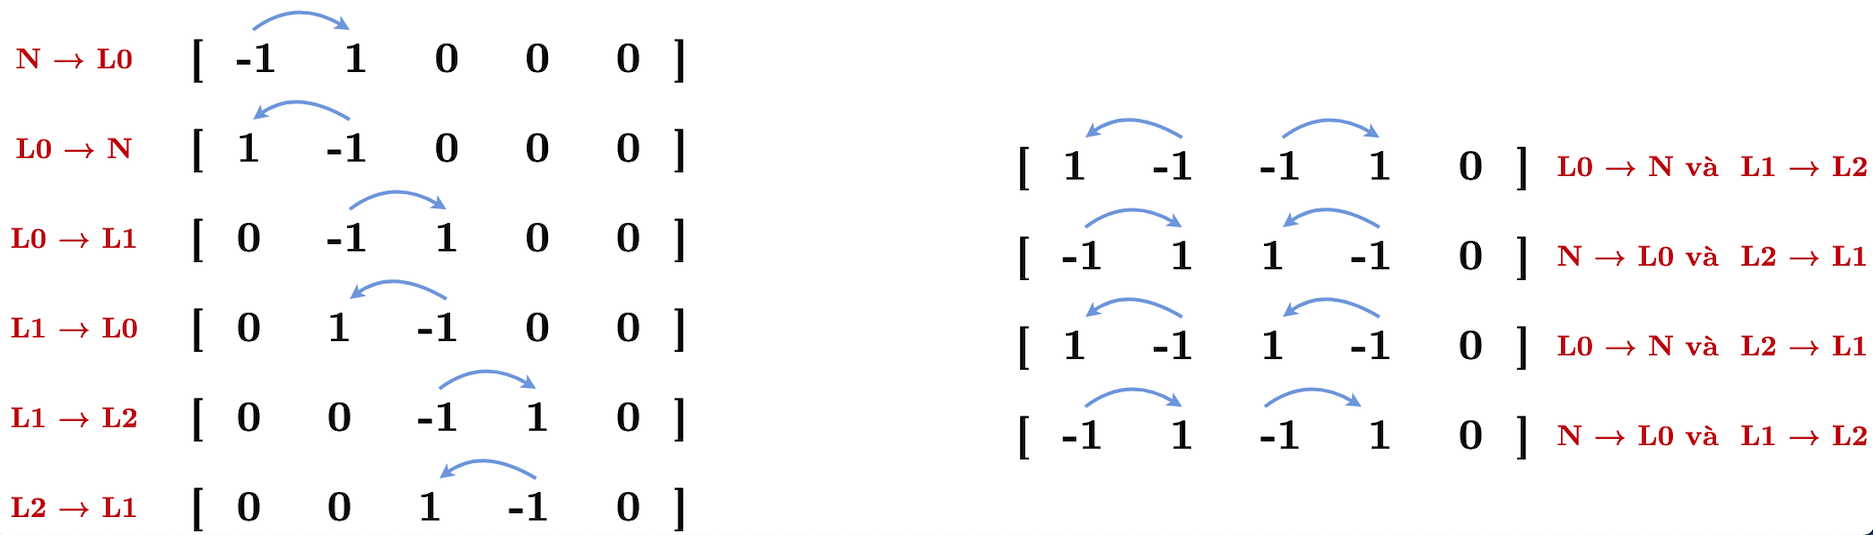
\includegraphics[width=0.8\textwidth]{source/1.png}\\
\vspace{8pt}
\textbf{\small Trường hợp không thoả mãn}\\
\vspace{2pt}

\includegraphics[width=0.6\textwidth]{source/2.png}\\
\end{center}
\end{frame}

\begin{frame}{Điều kiện dừng}{\secname}
\begin{columns}
\begin{column}{0.4\textwidth}
\begin{itemize}
\setlength\itemsep{8pt}
\item Khi hệ thống chạy được một khoảng thời gian là \keyword{\textcolor{mainblue}{\lstinline{container_lifetime = 43200}}}.
\item Trường hợp thiếu tài nguyên (phần trăm sử dụng CPU hay GPU lớn hơn 1), hoặc xảy ra hiện tượng tràn RAM 
\item[] $ \rightarrow $ Container được đưa về state nào không sử dụng tài nguyên tương ứng gần nhất.
\end{itemize}
\end{column}
\begin{column}{0.5\textwidth}
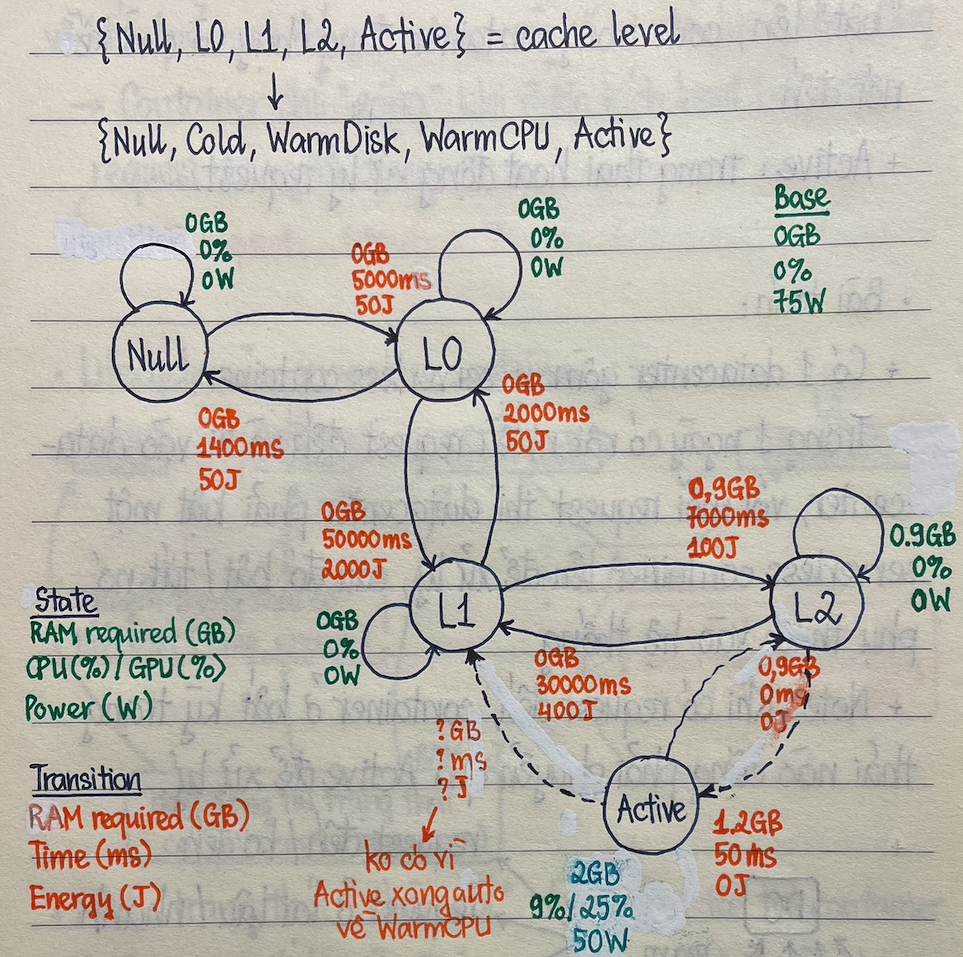
\includegraphics[width=0.88\textwidth]{source/3.png}\\
\end{column}
\end{columns}
\end{frame}

\begin{frame}{Kịch bản mô phỏng [Chỉnh sửa]}
\begin{itemize}
\setlength\itemsep{8pt}
\item Hệ thống khởi tạo ngẫu nhiên số lượng container và thời gian xử lý request ở mỗi service.
\item Hệ thống có số service là 4 (\keyword{\textcolor{mainblue}{\lstinline{size = 4}}}), tức ma trận container có 4 hàng.
\item Hệ thống nhận request đến tuân theo phân phối Poisson với $ \lambda = 100 $ \\
      (100 request/h; 1h = 3600s).
\item Mỗi 10 giây, hệ thống sẽ tính toán reward và các giá trị info (lượng RAM sử dụng, năng lượng tiêu thụ, profit...).
\item Mỗi 1 giây, thực hiện kiểm tra lượng container ở trạng thái WarmCPU có trong mỗi service và so sánh với lượng request:
\begin{itemize}
\setlength\itemsep{4pt}
\item[-] Nếu $ n_{WarmCPU} \geq n_{request} $ thì $ n_{WarmCPU} -= n_{request} $ rồi đặt $ n_{request} = 0 $, sau đó chờ thời gian xử lý, tính toán các tham số đánh giá, rồi cộng trở lại lượng WarmCPU vừa trừ.
\item[-] Nếu $ n_{WarmCPU} < n_{request} $ thì $ n_{request} -= n_{WarmCPU} $ rồi đặt $ n_{WarmCPU} = 0 $, lượng request dư ra được đưa vào hàng chờ, sau đó xử lý tương tự như trường hợp trên.
\end{itemize}
\end{itemize}
\end{frame}

\begin{frame}{Kịch bản mô phỏng [Chỉnh sửa]}
\begin{itemize}
\setlength\itemsep{8pt}
\item Công thức tính reward tối giản: 
\begin{equation*}
Reward = n_{request-in-L2} - \alpha \times t_{transition} - \beta \times Energy_{cost}
\end{equation*}
\item Điều kiện: 
\begin{itemize}
\setlength\itemsep{4pt}
\item[-] $ \alpha = 0.4, \, \beta = 0.02 $
\item[-] $ n_{request-in-L2} \leq n_{total-container} $
\item[-] Nếu $ t_{transition} < t_{timeout} $ thì request được xử lý, nếu $ t_{transition} \geq t_{timeout} $ thì request lỗi.
\end{itemize}
\item Mỗi 10 giây, thực hiện thêm việc kiểm tra các container có đang chuyển trạng thái hay không (dùng ma trận \keyword{\textcolor{mainblue}{\lstinline{_transition_matrix}}}) và thực hiện đưa ra action phù hợp:
\begin{itemize}
\setlength\itemsep{4pt}
\item[-] Nếu container đang chuyển trạng thái thì bỏ qua việc đưa ra action cho container này.
\item[-] Nếu container không chuyển trạng thái (chuyển trạng thái đã xong) thì đưa ra action.
\end{itemize}
\end{itemize}
\end{frame}

\section{Triển khai mô phỏng và đánh giá}

\subsection{Kết quả mô phỏng}

\begin{frame}{Kết quả mô phỏng}
\begin{center}
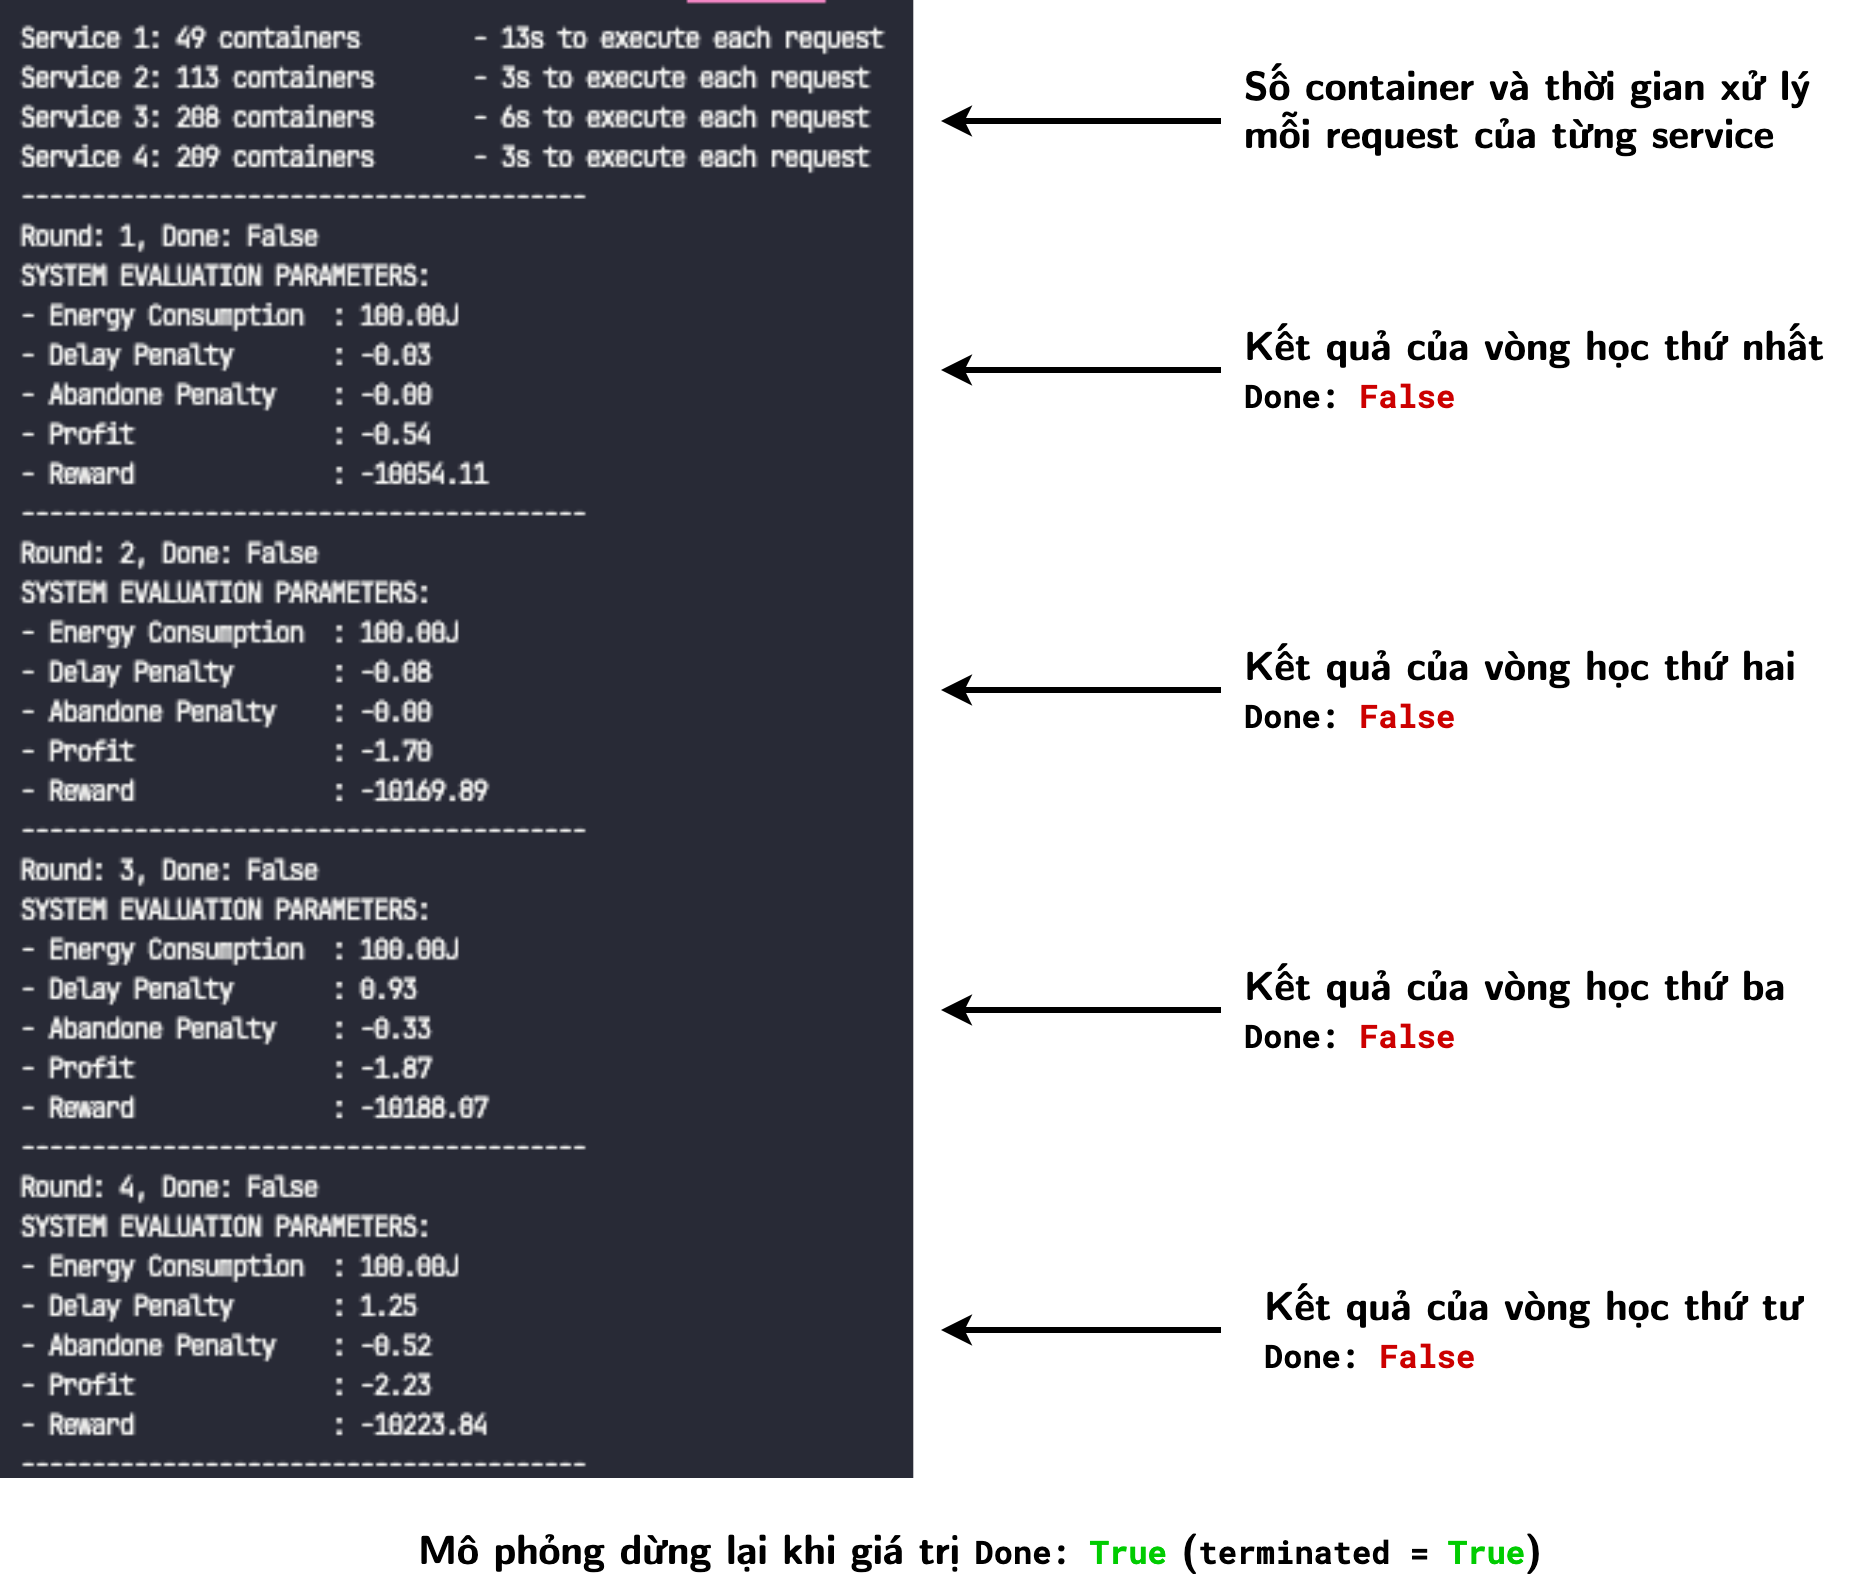
\includegraphics[width=0.54\textwidth]{source/5.png}\\
\end{center}
\end{frame}

\subsection{Đánh giá mô phỏng}

\begin{frame}{Nhận xét kết quả}{\subsecname}
\begin{itemize}
\setlength\itemsep{8pt}
\item Đôi lúc mô phỏng chỉ chạy được 1-2 vòng học rồi dừng lại.
\item[] $ \longrightarrow $ \textbf{Nguyên nhân:} Điều kiện xác định \keyword{\textcolor{mainblue}{\lstinline{terminated}}} chưa chặt chẽ, hoặc do lập trình sai.
\item Mô phỏng chạy bị lỗi, thỉnh thoảng mới chạy được =)))
\item[] $ \longrightarrow $ \textbf{Nguyên nhân:} Một số hàm và điều kiện được định nghĩa chưa chặt chẽ, sửa thêm.
\end{itemize}
\end{frame}

\begin{frame}{Vấn đề gặp phải (1)}{\subsecname}
\begin{itemize}
\setlength\itemsep{8pt}
\item Đang tìm hiểu cách tính reward theo cập nhật mềm, chưa áp dụng được trong mô phỏng.\\
\begin{center}
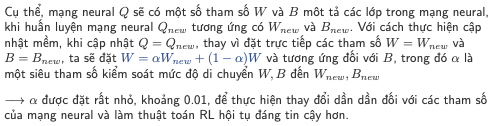
\includegraphics[width=0.8\textwidth]{source/4.png}\\
\end{center}
\item Luồng thời gian xử lý có thể bị sai (chưa rõ).
\end{itemize}
\end{frame}

\begin{frame}{Vấn đề gặp phải (2)}{\subsecname}
\begin{itemize}
\setlength\itemsep{8pt}
\item Tính $ Penalty_{delay} $ và $ Penalty_{abandone} $ chưa đúng? Hiểu sai?
\item Tính toán năng lượng $ Energy_{cost} $ chưa đúng? Lập trình sai?
\item Tính toán các tham số chuyển state chưa đúng?
\end{itemize}
\end{frame}

\section{Kết luận}

\begin{frame}{Kết luận}
\begin{itemize}
\setlength\itemsep{8pt}
\item Link Github mô phỏng: \textit{
\href{https://github.com/owofuyuki/reinforcement-learning-for-serverless}{https://github.com/owofuyuki/reinforcement-learning-for-serverless}}
\item Kết quả mô phỏng chưa đánh giá được vấn đề cho bài toán.
\item Chỉnh sửa mô phỏng...
\end{itemize}
\end{frame}

\backmatter

\end{document}